\documentclass{standalone}
\usepackage{tikz}
\begin{document}
	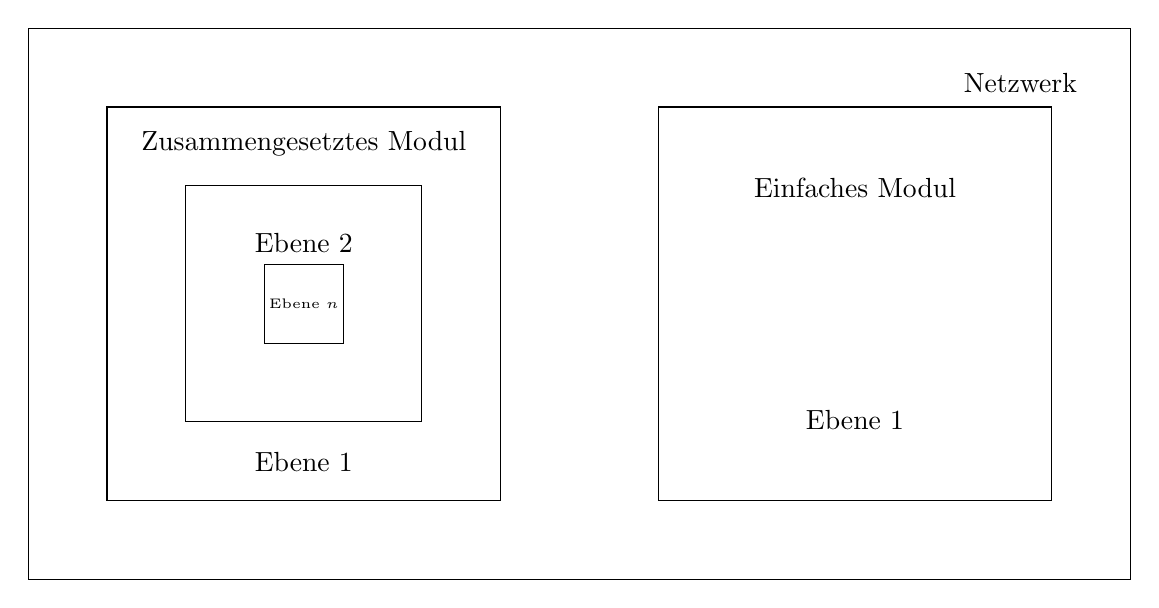
\begin{tikzpicture}	
		\draw (0,0) rectangle (14,7) node[pos=.9] {Netzwerk};
		\draw (1,1) rectangle (6,6) node[pos=.5, above=50] {Zusammengesetztes Modul} node[pos=.5, below=50] {Ebene 1};
		\draw (2,2) rectangle (5,5) node[pos=.5, above = 15] {Ebene 2};
		\draw (3,3) rectangle (4,4) node[pos=.5] {\tiny Ebene $n$};
		
		\draw (8,1) rectangle (13,6) node[pos=.5, above=35] {Einfaches Modul} node[pos=.5, below=35] {Ebene 1};
	\end{tikzpicture}
\end{document}